\chapter{Data Selection}
\label{cha:data_selection}

\section{Structure and size of data}
The selected dataset onto which a classification model shall be learned is provided by Kaggle \footnote{2017 Kaggle Inc}. It is named \textit{The movies Dataset}\footnote{Link to the dataset: \hyperref[https://www.kaggle.com/rounakbanik/the-movies-dataset]{https://www.kaggle.com/rounakbanik/the-movies-dataset}} and contains metadata on approximately 45,000 movies in its raw format. It is provided and updated by Rounik Banik. The complete dataset consits out of several files in the \textit{.csv} format containing specific info about movie casts, metadata, and external scores. For the outcome of this project the central file, used for further preprocessing is named \textit{movies-metadata.csv}. This csv-file holds 24 columns in total, which can be expected in the graphic below.
\begin{figure}[ht]
	\centering
		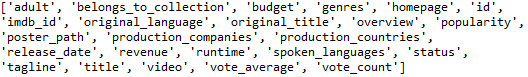
\includegraphics[width=\textwidth]{images/Raw_dataset_headers.png}
	\caption{Columns of the file \textit{movies-metadata.csv}}
\end{figure}

%Due to the multitude of attributes, it is essential to extract the relevant values for the implementation of a well-functioning classifier. Many values have no effect on the financial success of a movie and can therefore be ignored. This includes, for example, the columns...

The structure of the individual attributes is very different. In addition to boolean values, strings and numeric float values (e.g \textit{budget} or \textit{runtime}), many attributes contain longer texts (e.g \textit{overview}), arrays or even a list of JSON objects (e.g.\textit{production-countries} )These different formats must be taken into account in the later preprocessing step and need to be processed individually, so that a well-functioning classification model can be worked out.


\section{Basic data exploration}
If you take a closer look at the data it can be noticed that the overall quality varies significantly. This can be attributed to the fact that the record is maintained by a community and is not provided by a larger organization or company. Therefore, a demanding quality assurance process is difficult to realize. One  quality issue and special case is for example the encoding of string attributes of Asian movies and the Chinese and Japanese character set. Another aspect of importance is the absence of a lot of values. Especially for older movies (before 1960) there are just a few information available. This lack of information needs to be taken into account for the further steps. The most critical effect has the absence of values to numerical attributes like \textit{revenue} or \textit{budget}, which are also critical for the success of a classification model with respect to financial interests. Here around 34000 records are containing a zero or nothing in either the revenue or the budget column, what decimates the dataset heavily. 

In addition to that, there is no information about the currencies of financial attributes. Complicated because later computations will rely heavily on revenue and budget data. Average budget value, average revenue (without zero). Correlation between revenue and budget. The most common genre is... . Average number of actors per movie.

Back to revenue and budget take into account that this is data from past 60 years. A lot of things changed in movie economics (prices, consumer Verhalten, globalization). Introduced new column, productivity value
A lot of values are scaled wrongly. Little example with 2 movies. 2000000 in revenue is just stated as 2, don't know the scale of data. Will be a big problem


Main issue quality of data. Further explained in preprocessing...
